% ******************************************************** %
%              TEMPLATE DE INFORME ORGA2 v0.1              %
% ******************************************************** %
% ******************************************************** %
%                                                          %
% ALGUNOS PAQUETES REQUERIDOS (EN UBUNTU):                 %
% ========================================
%                                                          %
% texlive-latex-base                                       %
% texlive-latex-recommended                                %
% texlive-fonts-recommended                                %
% texlive-latex-extra?                                     %
% texlive-lang-spanish (en ubuntu 13.10)                   %
% ******************************************************** %


\documentclass[a4paper,]{article}
\usepackage[spanish]{babel}
\usepackage[utf8]{inputenc}
\usepackage{charter}   % tipografia
\usepackage{graphicx}
\usepackage[table,xcdraw]{xcolor}
%\usepackage{makeidx}
\usepackage{paralist} %itemize inline

\usepackage{float}
\usepackage{amsmath, amsthm, amssymb}
\usepackage{amsfonts}
%\usepackage{sectsty}
%\usepackage{charter}
%\usepackage{wrapfig}
\usepackage{listingsutf8}

% \setcounter{secnumdepth}{2}
\usepackage{underscore}
\usepackage{caratula}
\usepackage{url}
%\usepackage[superscript,biblabel]{cite}
%\usepackage{dibujitos}

\usepackage{amssymb}


\graphicspath{ {img/} {../graph/} }

% ********************************************************* %
% ~~~~~~~~              Code snippets             ~~~~~~~~~ %
% ********************************************************* %

\usepackage{color} % para snipets de codigo coloreados
\usepackage{fancybox}  % para el sbox de los snipets de codigo

\definecolor{litegrey}{gray}{0.94}

\newenvironment{codesnippet}{%
	\begin{Sbox}\begin{minipage}{\textwidth}\sffamily\small}%
	{\end{minipage}\end{Sbox}%
		\begin{center}%
		\vspace{-0.4cm}\colorbox{litegrey}{\TheSbox}\end{center}\vspace{0.3cm}}

\definecolor{mygreen}{rgb}{0,0.6,0}
\definecolor{mygray}{rgb}{0.5,0.5,0.5}
\definecolor{mymauve}{rgb}{0.58,0,0.82}

\lstset{ %
  backgroundcolor=\color{litegrey},
  basicstyle=\footnotesize,
  breakatwhitespace=true,
  breaklines=true,
  captionpos=b,                    % sets the caption-position to bottom
  mathescape=true,
  keepspaces=true,
  language=Python,
  showspaces=false,
  tabsize=2,                       % sets default tabsize to 2 spaces
  inputencoding=utf8/latin1
}

\newcommand{\cuidado}{{\large $\Delta$!!!} \hspace*{1em}}

\newcommand*{\QEDA}{\hfill\ensuremath{\blacksquare}}%
\newcommand*{\QEDB}{\hfill\ensuremath{\square}}%

% ********************************************************* %
% ~~~~~~~~         Formato de las páginas         ~~~~~~~~~ %
% ********************************************************* %

\usepackage{fancyhdr}
\pagestyle{fancy}

\renewcommand{\sectionmark}[1]{\markright{\thesection\ - #1}}

\fancyhf{}

\fancyhead[LO]{Sección \rightmark} % \thesection\
\fancyfoot[LO]{\small{Agustín Borgna, Cristian Vazquez, Gian Franco Lancioni, Juan Gonzalez Benitez - \textbf{Redes (TP2)}}}
\fancyfoot[RO]{\thepage}
\renewcommand{\headrulewidth}{0.5pt}
\renewcommand{\footrulewidth}{0.5pt}
\setlength{\hoffset}{-0.8in}
\setlength{\textwidth}{16cm}
%\setlength{\hoffset}{-1.1cm}
%\setlength{\textwidth}{16cm}
\setlength{\headsep}{0.5cm}
\setlength{\textheight}{25cm}
\setlength{\voffset}{-0.7in}
\setlength{\headwidth}{\textwidth}
\setlength{\headheight}{13.1pt}

\renewcommand{\baselinestretch}{1.1}  % line spacing

% ******************************************************** %


\begin{document}


\thispagestyle{empty}
\materia{Teoría de las Comunicaciones}
\submateria{Primer Cuatrimestre de 2017}
\titulo{Trabajo Práctico 1}
\subtitulo{Rutas en Internet}
\integrante{Borgna, Agustín}{079/15}{aborgna@dc.uba.ar}
\integrante{Gonzalez Benitez, Juan}{324/14}{gonzalezjuan.ab@gmail.com}
\integrante{Lancioni, Gian Franco}{234/15}{gianflancioni@gmail.com}
\integrante{Vazquez, Cristian}{056/10}{cristianvazquez4@gmail.com}

\maketitle
\newpage

\thispagestyle{empty}
\vfill

\thispagestyle{empty}
\vspace{2cm}
\tableofcontents
\newpage


\normalsize
\newpage
\twocolumn
A modo muy general, con el objetivo de analizar distintas redes locales, vamos a modelar ciertos comportamientos en el tráfico como fuentes de Teoría de la Información y poder extraer conclusiones concretas partiendo de las herramientas conocidas, particularmente los conceptos de entropía de la fuente e información de un símbolo en dicha fuente, para estudiar dichas fuentes.
\section{Introducción}
\subsection{ARP}
En particular nos interesa analizar las interacciones que se dan entre hosts de la red con el fin resolver direcciones de capa de red hacia capa de enlace, usualmente IP a MAC. Estas interacciones son propias del \emph{ARP (protocolo de resolución de direcciones)} \footnote{https://en.wikipedia.org/wiki/Address_Resolution_Protocol}, el cual cumple un rol crucial en lo que conocemos como \emph{internetworking}.

Se trata de un protocolo de \emph{request} y \emph{response}, implementados a partir de paquetes \emph{'who-has'}, que preguntan a un dominio de broadcast por la \emph{MAC address} de una IP particular, y paquetes \emph{'is-at'} que responden de manera unicast al emisor del paquete 'who-has'.

El tipo del paquete se determina por el campo de operación de dicho paquete, del cual haremos amplio uso.

Por supuesto, dicho protocolo no se ejecuta cada vez que se quiera efectuar una transmisión, sino que los resultados se almacenan temporalmente una \emph{cache} para agilizar tiempos.

\subsection{Herramientas y resolución de primer etapa}
Cada una de las capturas de red que hicimos (una por cada integrante del grupo), se hizo con el programa \emph{TShark}, versión \emph{terminal-based} del packet sniffer \emph{Wireshark}.

Los paquetes obtenidos los manipulamos con el framework \emph{Scapy} de \emph{Python} que nos permite acceder a los campos de cada uno y, por ejemplo, determinar si tiene capa \emph{ARP} y (de ser así) su destino buscado.

\subsubsection{Primer ejercicio}

Lo primero que se nos pide es modelar cada red como una fuete de información binaria $S$ de memoria nula con símbolos en $\{S_{unicast},\ S_{broadcast}\}$.

Para implementar la fuente simplemente contaremos la cantidad de paquetes $p$ tales que $p.dst =$ 'ff:ff:ff:ff:ff:ff' (i.e la dirección MAC de destino de broadcast). Dicha implementación está en \emph{entro.py} y se encarga de imprimir por pantalla la entropía de la fuente y las ocurrencias de cada símbolo para una secuencia dada de paquetes.

Por lo tanto dicha fuente se abstrae de la identidad de los nodos de la red y los trata indiscriminadamente como emisores de símbolos según la dirección de capa de enlace de sus paquetes.

A modo analítico, la fuente $S$ de cada red permite entender de qué manera se comunican los hosts de la red.

Por ejemplo, al tratarse de conexiones predominantemente dirigidas, resultaría extraño que los paquetes de broadcast fueran mayoría en el tráfico de la red. Y en caso contrario, la fuente haría visibles escenarios particulares de topologías o comunicaciones entre hosts.

\subsubsection{Segundo ejercicio}

El segundo ejercicio consistió en modelar una nueva fuente de información $S_1$ de memoria nula, con el objetivo de distinguir, en lugar de tipos de destinos como lo hacía $S$, los propios nodos (hosts) de la red.

Dicha distinción se hizo a partir de los paquetes \emph{ARP}, y la implementación se encuentra en \emph{distinguidos.py}.

Lo que hicimos fue considerar como símbolos las \emph{IPs} de request de los mensajes 'who-has'. De esta manera, los símbolos con menos información son aquellos más solicitados.

Entonces los nodos distinguidos, con la finalidad de exponer aquellos más 'importantes' en la red, los consideramos como aquellos símbolos $s$ tales que $I(s) < H(S_1)$ siendo $I(s)$ la información del nodo s en la fuente $S_1$ y $H(S_1)$ la entropía de la fuente.

Siguiendo con esta idea, es de esperarse que los nodos más solicitados, como los \emph{default gateways} aparezcan siempre entre los distinguidos.

\newpage
\onecolumn
\section{Mediciones realizadas}
Ahora mostraremos los datos obtenidos en todas las mediciones, considerando las herramientas obtenidas en los dos ejercicios de la primera etapa mas un conjunto de gráficos que aporten nuevos datos para poder analizar.

\subsection{University of London}
\label{sec:london}

Para esta medición se eligió la Universidad de Londres (King's College, the London School of Economics and Political Science, etc), ubicada en Londres, Inglaterra. El destino propiamente dicho es \emph{'london.ac.uk'}. Se esperaría encontrar dos tramos transatlánticos: Argentina-Miami y uno transatlántico, asumiendo paso intermedio por EEUU. Hicimos las mediciones varias veces en días aledaños y los resultados fueron siempre consistentes.  Midiendo de a 30 iteraciones por TTL observamos los siguientes RTTs:
\\

\begin{figure}[H]
    \centering
    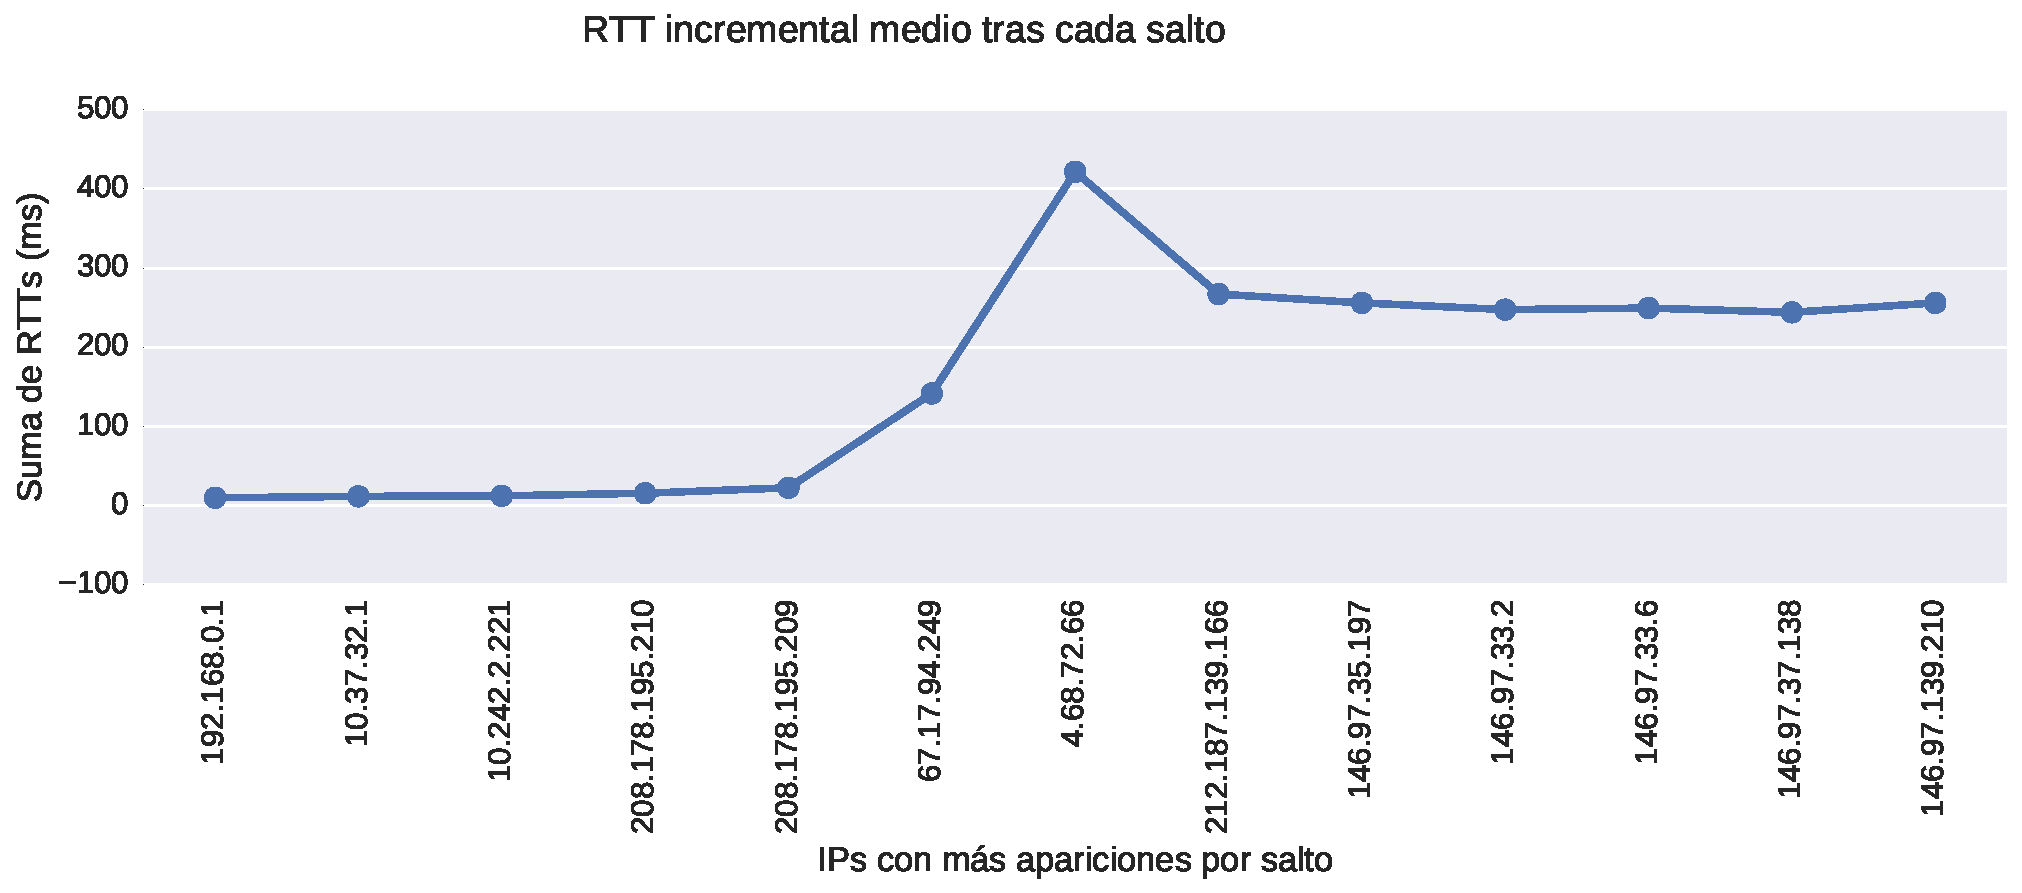
\includegraphics[width=1\textwidth, height=1\textheight, keepaspectratio]{../img/lan-incrementales}
    \caption{Comportamiento incremental de RTTs medios medidos.}
    \label{fig:lan-incrementales}
\end{figure}

Se notan dos tramos donde las diferencias entre RTTs relativos son bajas y constantes, que seguramente se corresponden al entramado interno de Buenos Aires y Londres en contraste con las rutas submarinas con mayores promedios.

\begin{figure}[H]
   \centering
       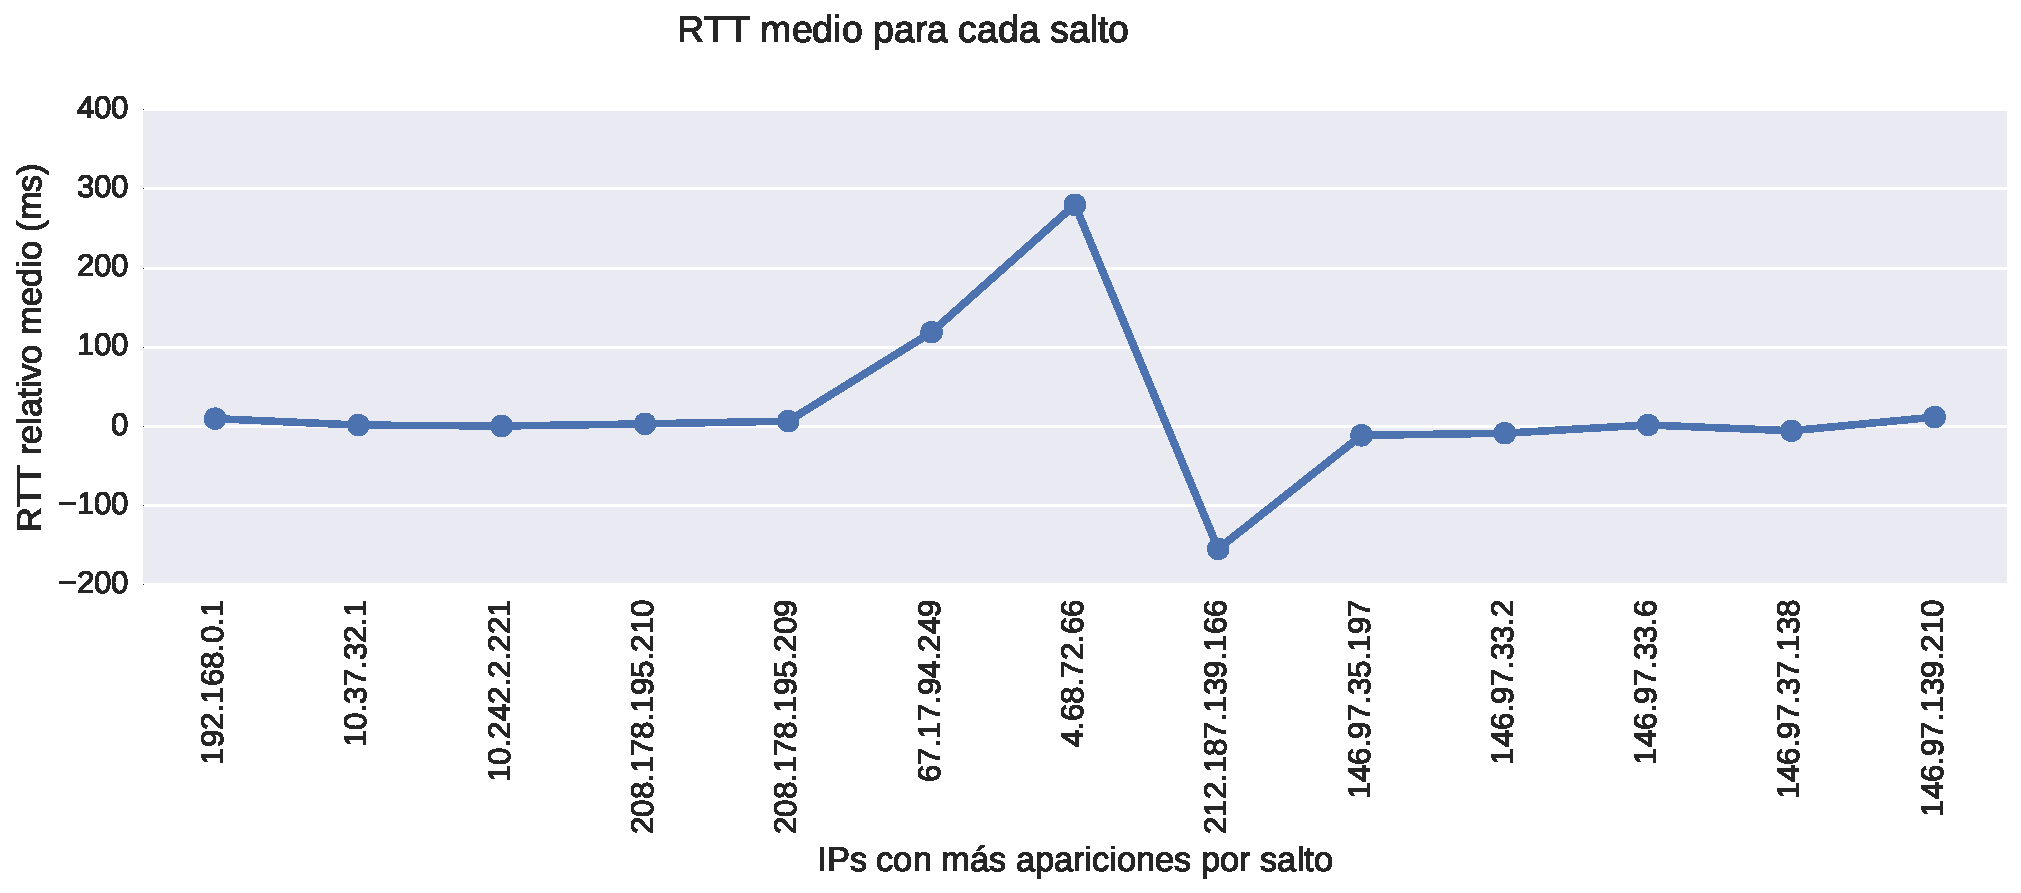
\includegraphics[width=1\textwidth, height=1\textheight, keepaspectratio]{../img/lan-rtts}
 \caption{RTTs medios medidos para una traceroute a la Universidad de Londres.}
 \label{fig:lan-rtts}
\end{figure}


Se pueden observar un gateway que conforma un pico, adjudicado a las IPs '4.68.72.66' geolocalizada en Estados Unidos con hostname \emph{'lag-9.ear1.Miami1.Level3.net'}. Podemos suponer que se trata de un gateway extremadamente cargado, posiblemente por estar en una red troncal respecto a enlaces submarinos. Este es el único nodo que cambió entre mediciones, dado que en las repeticiones posteriores y anteriores no era común su aparición, que quizás se deba a algún rebalanceo. \\


Anteriores a este salto aparecen dos nodos interesantes que son el '208.178.195.209' y '67.17.94.249', ambos adjudicados a Estados Unidos.
La '208.178.195.209' destaca porque, al igual que '208.178.195.210' tiene una latencia sospechosamente similar a las locales de Argentina. Mientras que la '67.17.94.249' presenta un gran salto respecto de su anterior en términos de RTT.

Por lo cual se especula que '208.178.195.210' y '208.178.195.209' son gateways locales, partes del backbone argentino que conecta con links internacionales. Lo cual se condice con el hostname de la última: \emph{'global-crossing-argentina-s-a.xe-0-1-0.ar3.eze1.gblx.net'}.

Esto significaría que '67.17.94.249' es el gateway del lado estadounidense del link intercontinental. \\

El nodo '212.187.139.166' es el primero adjudicado a Londres, siendo candidato a extremo británico del enlace transatlántico. Tiene promedio negativo, esto no sorprende, dado que su antecesor ('4.68.72.66') tenía un promedio muy alto.

\begin{figure}[H]
   \centering
       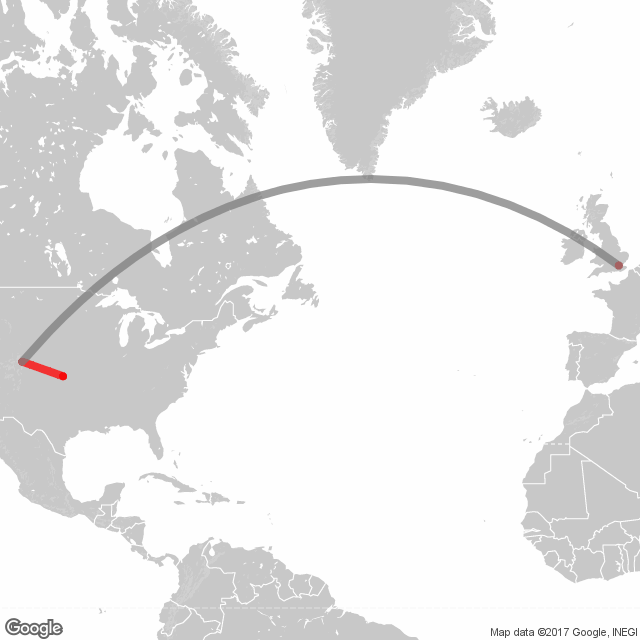
\includegraphics[width=0.5\textwidth, keepaspectratio]{../img/lan-map}
 \caption{Mapa de ubicaciones inferidas para una traceroute a la Universidad de Londres.}
 \label{fig:lan-map}
\end{figure}

Se puede notar el enlace transatlántico mencionado antes, y en rojo fuerte el gateway sobrecargado de Estados Unidos.

El traceroute presenta algo curioso, y es que todos los nodos locales a Argentina tienen asignadas IPs reservadas/privadas (192.168.0.1, 10.37.32.1, 10.242.2.221). Por lo tanto el geolocalizador solamente puede empezar a reconocer nodos a partir de las IPs estadounidenses (que, como dijimos anteriormente, las primeras están mal adjudicadas dado que probablemente estén ubicadas en el extremo argentino del enlace Argentina-Miami) significando que en el mapa el punto de origen se encuentra en dicho país. \\

Respecto al porcentaje de nodos que respondieron los \emph{requests} sucede otra anomalía: el host destino parecería no estar configurado para emitir respuestas de este tipo. Esto implica que el traceroute sigue emitiendo hasta llegar al límite preestablecido de los 30 \emph{hoops}, y no poder determinar con total seguridad en qué salto se llega al destino (y cuántos en el medio no respondieron).

Asumiendo que es el último en responder (responde por \emph{time-exceeded}, no \emph{echo-reply}), el porcentaje sería aproximadamente del \textbf{93\%} con un único nodo mudo ubicado entre '67.17.94.249' y '4.68.72.66', es decir en el backbone estadounidense.



\begin{figure}[H]
   \centering
       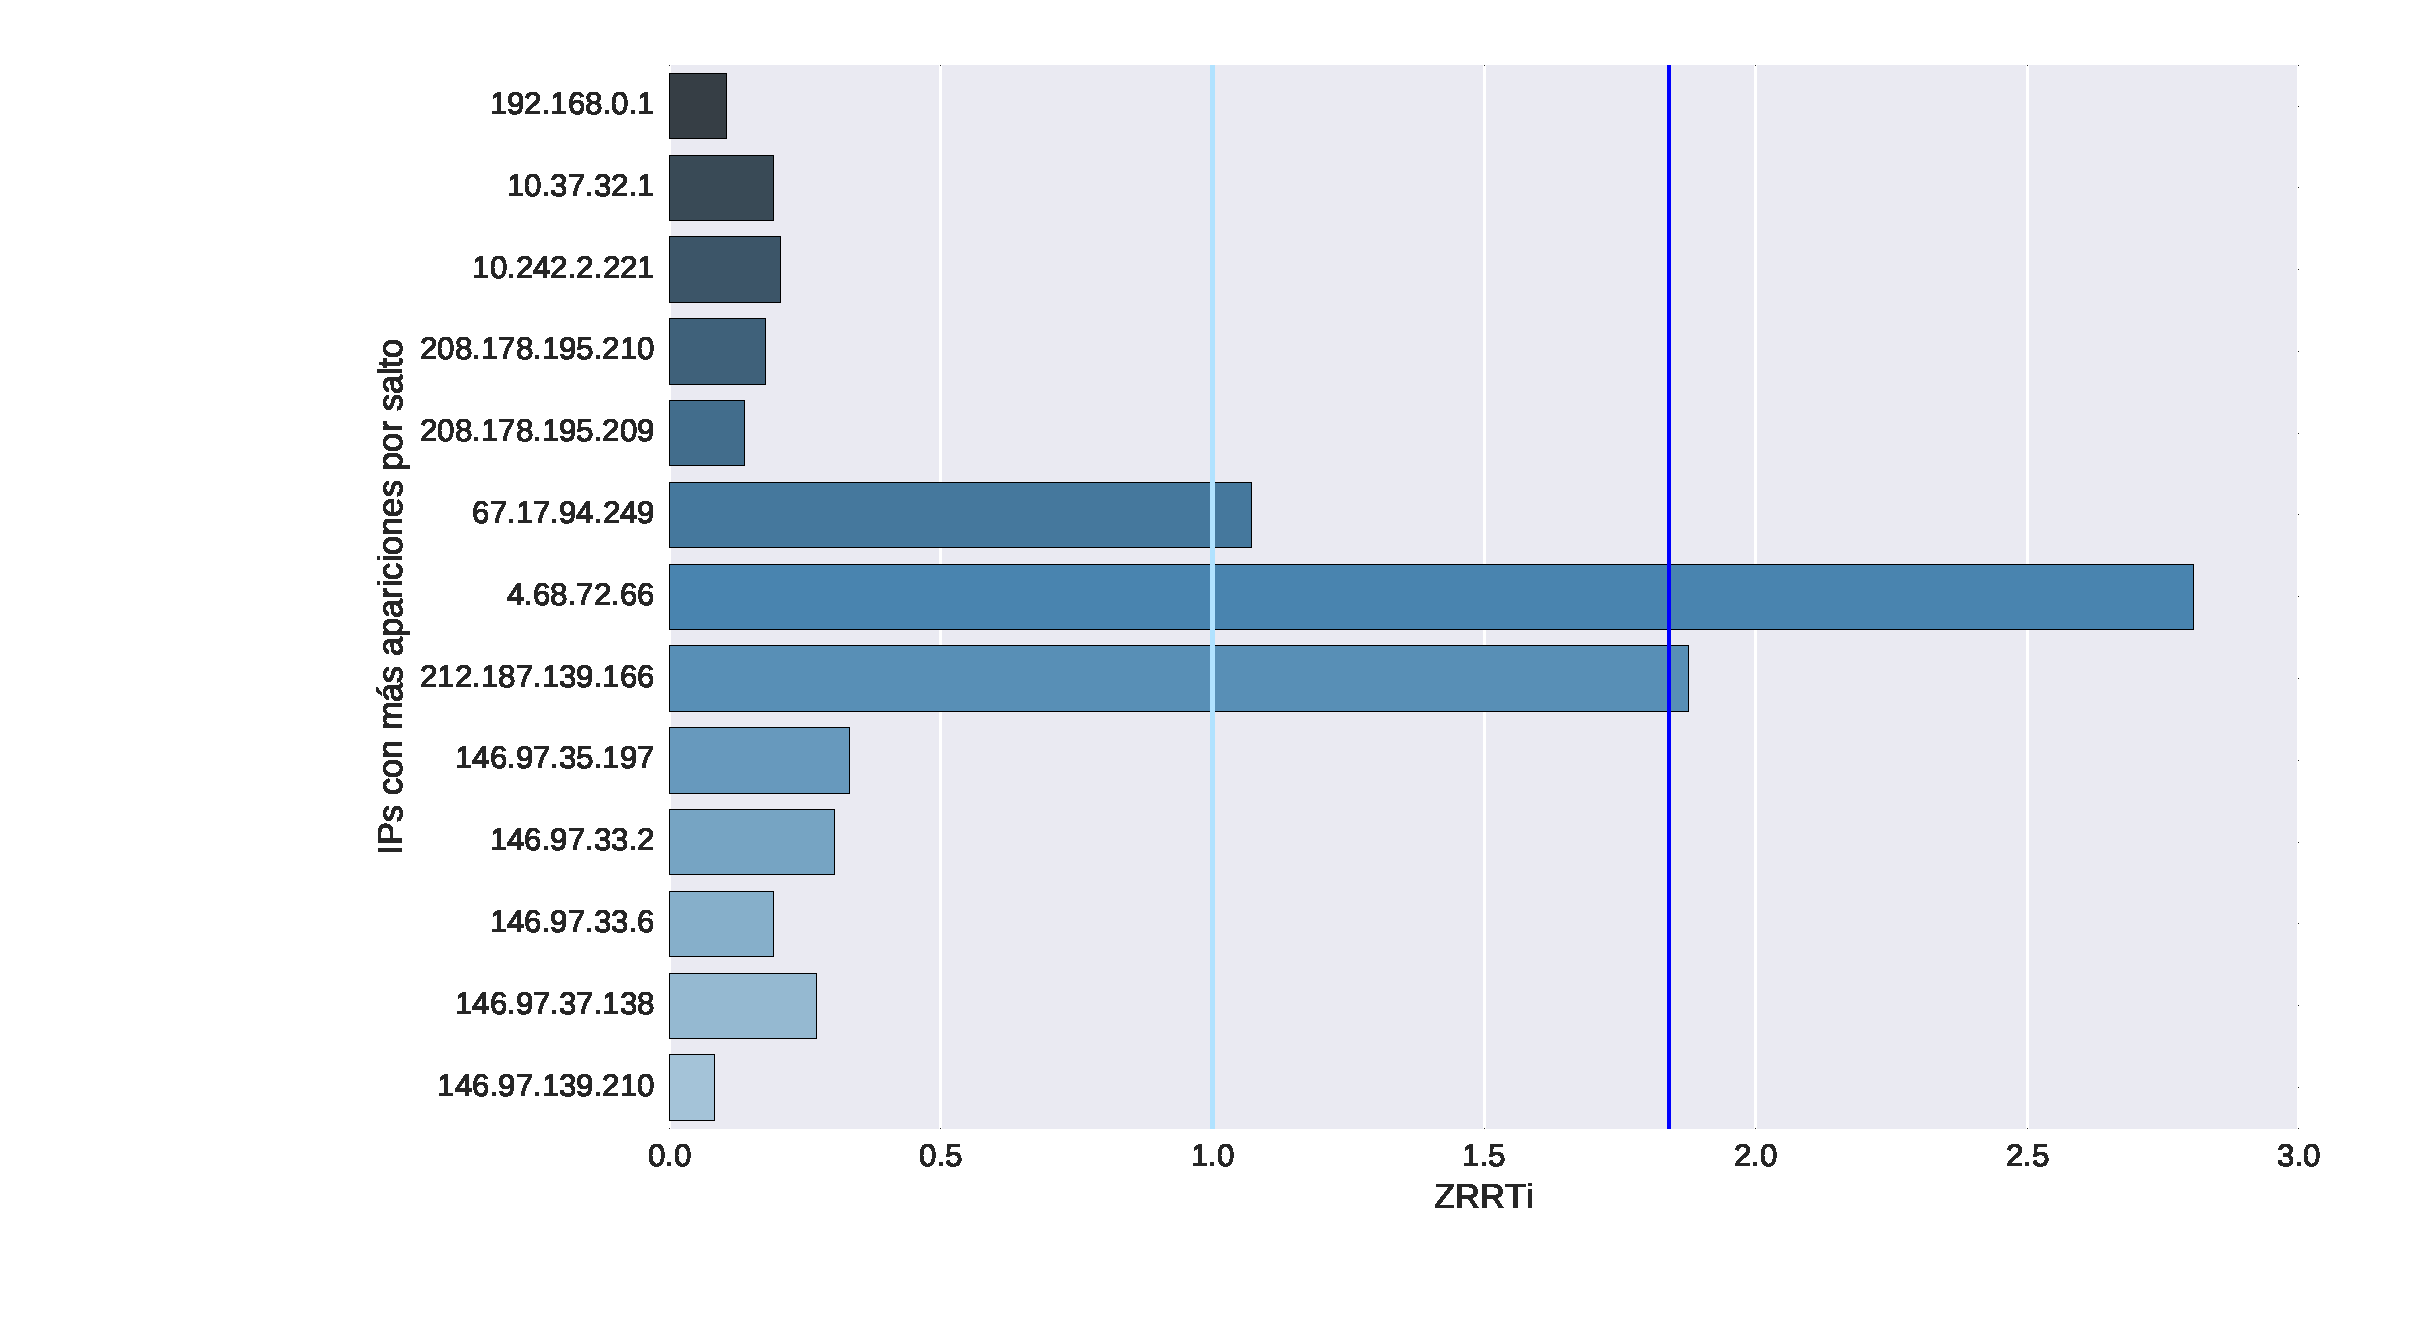
\includegraphics[width=1\textwidth, height=1\textheight, keepaspectratio]{../img/lan-zrtt}
 \caption{Outliers de la distribución ZRRTi según el método de Cimbala. En azul oscuro: valor $ZRTT_i$ correspondiente a $\tau(n)$ con $n$ el largo de ruta y un alfa fijo (0.05 sugerido en el paper de referencia).}
 \label{fig:lan-zrtt}
\end{figure}

En la figura \ref{fig:lan-zrtt} se ven los outliers de la muestra. Respecto del umbral de la tabla $\tau$, se distinguen los nodos del extremo británico del transatlántico y el gateway sobrecargado de EEUU, que no es extremo intercontinental pero sí presentó muchísima latencia. \\

El otro extremo intercontinental que falta, el de Argentina-Miami aparece con el umbral $Z=1$ (es decir aquellos que están por encima de la desviación estándar normalizada) junto a los dos anteriores, pasando de un falso negativo y un falso positivo, a un único error del tipo falso positivo para el nodo en sobrecarga. Por lo tanto el modelado de la distribución es relativamente exitoso para encontrar dichos tramos, aunque el gateway más destacado no sea un tramo intercontinental.

\newpage
\section{Conclusiones Generales}
En general, todas las mediciones pudieron detectar al menos un cable intercontinental. Generalmente aquellos transoceánicos con grandes latencias. La fiabilidad de las rutas la pudimos contrastar con la implementación de Unix para traceroutes (implementada sobre UDP) y corroboramos que los resultados eran similares.

Sin embargo, pudimos notar muchas anomalías de diversos tipos.
\\

Una de las primeras anomalías con las que nos encontramos fue que aparecían IPs de España en el tramo Argentina-Miami en la medición de Nueva Zelanda, lo cual suponemos que esté relacionado a una asignación de IPs particular del ISP. Pero esto significó, desde la primer medición, entender la falibilidad natural de cualquier herramienta de geolocalización de IPs respecto a nuestras expectativas de que el entramado final siempre sea consistente. Lo cual se profundizó a medida que fuimos encontrando nodos geolocalizados en un extremo de enlace intercontinental, pero con latencias propias del otro extremo.
\\

Otra anomalía interesante fue que a veces los hosts destino no respondieron \emph{echo-reply} al recibir el mensaje o nodos intermedios que no responden los \emph{time-exceeded}. Comúnmente, esto pasa porque hay un \emph{firewall} configurado para bloquear cierto tipo de comportamientos, en este caso de \emph{ICMP}. Usualmente es tanto para evitar \emph{smurf attacks (ICMP spoofing)\footnote{https://en.wikipedia.org/wiki/Smurf_attack}} como por motivos de performance. Lo cual quizás sea inesperado viniendo de universidades y no de empresas comerciales.
\\

Estuvieron presentes casos de falsos negativos y falsos positivos. Después de todo, la detección de enlaces de alta latencia como outliers se trata de una técnica probabilística y puede fallar. Razones simples para que esto suceda pueden ser que existan nodos que no conforman ningún extremo intercontinental en sobrecarga (como en el caso de la medición de Londres) o predominio de rutas de larga distancia con minoría de entramado local (como por ejemplo en la de Uzbekistán) que haga que la media de los ZRTT sea alta, y por lo tanto algunos cables de alta latencia no destaquen (en el ejemplo, Argentina-Miami) y algunos cables locales tengan un alto ZRTT por su bajo RTT respecto de la media inflada.

Otro motivo de falla, más natural y esperable, es el caso de la medición de Nueva Zelanda, donde el cable submarino entre Australia y Nueva Zelanda no presenta diferencias de RTT que ameriten un outlier.

\appendix

%\newpage
%\bibliography{bibliography}{}
%\bibliographystyle{plain}

\end{document}
